\documentclass{beamer}
\usepackage{amsmath}
\usepackage[english]{babel} %set language; note: after changing this, you need to delete all auxiliary files to recompile
\usepackage[utf8]{inputenc} %define file encoding; latin1 is the other often used option
\usepackage{csquotes} % provides context sensitive quotation facilities
\usepackage{graphicx} %allows for inserting figures
\usepackage{booktabs} % for table formatting without vertical lines
\usepackage{textcomp} % allow for example using the Euro sign with \texteuro
\usepackage{stackengine}
\usepackage{wasysym}
\usepackage{tikzsymbols}
\usepackage{textcomp}
\usepackage{xcolor}
\usepackage[dvipsnames]{xcolor}
\usepackage{colortbl}
\usepackage{adjustbox}
\usepackage{tikz} % allows drawing figures
\usetikzlibrary{decorations.pathreplacing}
\newcommand{\bubblethis}[2]{
        \tikz[remember picture,baseline]{\node[anchor=base,inner sep=0,outer sep=0]%
        (#1) {\underline{#1}};\node[overlay,cloud callout,callout relative pointer={(0.2cm,-0.7cm)},%
        aspect=2.5,fill=yellow!90] at ($(#1.north)+(-0.5cm,1.6cm)$) {#2};}%
    }%
\tikzset{face/.style={shape=circle,minimum size=4ex,shading=radial,outer sep=0pt,
        inner color=white!50!yellow,outer color= yellow!70!orange}}
%% Some commands to make the code easier
\newcommand{\emoticon}[1][]{%
  \node[face,#1] (emoticon) {};
  %% The eyes are fixed.
  \draw[fill=white] (-1ex,0ex) ..controls (-0.5ex,0.2ex)and(0.5ex,0.2ex)..
        (1ex,0.0ex) ..controls ( 1.5ex,1.5ex)and( 0.2ex,1.7ex)..
        (0ex,0.4ex) ..controls (-0.2ex,1.7ex)and(-1.5ex,1.5ex)..
        (-1ex,0ex)--cycle;}
\newcommand{\pupils}{
  %% standard pupils
  \fill[shift={(0.5ex,0.5ex)},rotate=80] 
       (0,0) ellipse (0.3ex and 0.15ex);
  \fill[shift={(-0.5ex,0.5ex)},rotate=100] 
       (0,0) ellipse (0.3ex and 0.15ex);}

\newcommand{\emoticonname}[1]{
  \node[below=1ex of emoticon,font=\footnotesize,
        minimum width=4cm]{#1};}
\usepackage{scalerel}
\usetikzlibrary{positioning}
\usepackage{xcolor,amssymb}
\newcommand\dangersignb[1][2ex]{%
  \scaleto{\stackengine{0.3pt}{\scalebox{1.1}[.9]{%
  \color{red}$\blacktriangle$}}{\tiny\bfseries !}{O}{c}{F}{F}{L}}{#1}%
}
\newcommand\dangersignw[1][2ex]{%
  \scaleto{\stackengine{0.3pt}{\scalebox{1.1}[.9]{%
  \color{red}$\blacktriangle$}}{\color{white}\tiny\bfseries !}{O}{c}{F}{F}{L}}{#1}%
}
\usepackage{fontawesome} % Social Icons
\usepackage{epstopdf} % allow embedding eps-figures
\usepackage{tikz} % allows drawing figures
\usepackage{amsmath,amssymb,amsthm} %advanced math facilities
\usepackage{lmodern} %uses font that support italic and bold at the same time
\usepackage{hyperref}
\usepackage{tikz}
\hypersetup{
    colorlinks=true,
    linkcolor=blue,
    filecolor=magenta,      
    urlcolor=blue,
}
\usepackage{tcolorbox}
%add citation management using BibLaTeX
\usepackage[citestyle=authoryear-comp, %define style for citations
    bibstyle=authoryear-comp, %define style for bibliography
    maxbibnames=10, %maximum number of authors displayed in bibliography
    minbibnames=1, %minimum number of authors displayed in bibliography
    maxcitenames=3, %maximum number of authors displayed in citations before using et al.
    minnames=1, %maximum number of authors displayed in citations before using et al.
    datezeros=false, % do not print dates with leading zeros
    date=long, %use long formats for dates
    isbn=false,% show no ISBNs in bibliography (applies only if not a mandatory field)
    url=false,% show no urls in bibliography (applies only if not a mandatory field)
    doi=false, % show no dois in bibliography (applies only if not a mandatory field)
    eprint=false, %show no eprint-field in bibliography (applies only if not a mandatory field)
    backend=biber %use biber as the backend; backend=bibtex is less powerful, but easier to install
    ]{biblatex}
\addbibresource{../mybibfile.bib} %define bib-file located one folder higher


\usefonttheme[onlymath]{serif} %set math font to serif ones

\definecolor{beamerblue}{rgb}{0.2,0.2,0.7} %define beamerblue color for later use

%%% defines highlight command to set text blue
\newcommand{\highlight}[1]{{\color{blue}{#1}}}


%%%%%%% commands defining backup slides so that frame numbering is correct

\newcommand{\backupbegin}{
   \newcounter{framenumberappendix}
   \setcounter{framenumberappendix}{\value{framenumber}}
}
\newcommand{\backupend}{
   \addtocounter{framenumberappendix}{-\value{framenumber}}
   \addtocounter{framenumber}{\value{framenumberappendix}}
}

%%%% end of defining backup slides

%Specify figure caption, see also http://tex.stackexchange.com/questions/155738/caption-package-not-working-with-beamer
\setbeamertemplate{caption}{\insertcaption} %redefines caption to remove label "Figure".
%\setbeamerfont{caption}{size=\scriptsize,shape=\itshape,series=\bfseries} %sets figure  caption bold and italic and makes it smaller

\newtcolorbox{boxA}{
    fontupper = \bf,
    boxrule = 1.5pt,
    colframe = black % frame color
}
\newtcolorbox{boxB}{
    boxrule = 1.5pt,
    colframe = blue!70!black,, % frame color
    colback = blue!7!white,
}
\usetheme{Boadilla}

% --------------------
% Overall information
% --------------------
\title[Economía I]{Economía I \vspace{4mm}
\\ Magistral 24: Mercado de dinero II}
\date{}
\author[Franco Riottini]{Riottini Franco}
\vspace{0.4cm}
\institute[]{Universidad de San Andrés} 


\begin{document}

\begin{frame}
\titlepage
\centering
Magistral 24

\includegraphics[scale=0.2]{../Figures/logoUDESA.jpg} 
\end{frame}

\begin{frame}{La teoría cuantitativa del dinero}

    \begin{block}{España y el oro de América}
        La llegada masiva de metales preciosos a Europa generó un aumento en la cantidad de dinero en circulación, lo que llevó a un incremento en los precios.
    \end{block}

    La respuesta de los economistas clásicos fue simple, pero revolucionaria:
    \[
    M \times V = P \times Y
    \]
    Donde:
    \begin{itemize}
        \item \(M\): cantidad de dinero en circulación,
        \item \(V\): velocidad de circulación del dinero,
        \item \(P\): nivel general de precios,
        \item \(Y\): producción real de la economía.
    \end{itemize}

    Si la cantidad de dinero crece más rápido que la producción, los precios suben. Si el dinero circula más rápido (por desconfianza, inflación esperada, digitalización), los precios suben también.

\end{frame}


\begin{frame}{¿Qué determina la inflación?}
    \textit{
    ¿Puede un país imprimir dinero para resolver todos sus problemas, o eso termina inevitablemente en inflación?
    }

    \vspace{1.2em}
    La teoría cuantitativa del dinero nos da una respuesta matemática y empírica:

    \[
    \frac{\Delta M}{M} + \frac{\Delta V}{V} = \frac{\Delta P}{P} + \frac{\Delta Y}{Y}
    \]

    Si la velocidad (\(V\)) y la producción (\(Y\)) no cambian mucho, entonces:

    \[
    \pi = \frac{\Delta M}{M} + \frac{\Delta V}{V} - \frac{\Delta Y}{Y}
    \]
    donde \(\pi\) es la inflación.

\end{frame}


% \begin{frame}{Evolución de la base monetaria vs. IPC}
% \centering\includegraphics[width=11cm]{../Figures/C33.4.jpg}\
% \end{frame}

\begin{frame}{Evolución de la base monetaria vs. IPC}
    \centering
    \includegraphics[width=11cm]{../Figures/C38.7.png}\
\end{frame}

% \begin{frame}{El equilibrio del mercado monetario}
% \centering\includegraphics[width=11cm]{../Figures/P56.png}\
% \end{frame}

\begin{frame}{Velocidad de circulación}
\centering\includegraphics[width=10cm]{../Figures/C38.10.png}\
\end{frame}

\begin{frame}{Teorías alternativas de la inflación}
    \begin{itemize}
        \item Muchas otras variables se mueven junto con la inflación y llevan a pensar que son la causa:
        \begin{itemize}
            \item Es la puja distributiva
            \item Es culpa del dolar
            \item El aumento de las tarifas como generadoras de inflación
            \item Los supermercados aumentan los márgenes de ganancia y eso explica por qué aumentan los precios
        \end{itemize}
        \item No debemos confundir causas intermedias con causas últimas
    \end{itemize}
\end{frame}

% \begin{frame}{La relación entre política monetaria y precios...}
% \centering\includegraphics[width=11cm]{../Figures/P57.png}\
% \end{frame}

% \begin{frame}{La relación entre tarifas e inflación...}
% \centering\includegraphics[width=11cm]{../Figures/G20.png}\
% \end{frame}


\begin{frame}{¿Por qué emitir dinero?}
    \begin{itemize}
        \item La inflación puede funcionar como variable de ajuste
        \item El gobierno se queda con el impuesto inflacionario
        \begin{itemize}
            \item Al emitir dinero, el gobierno hace que el salario de la gente valga menos
        \end{itemize}
        \item La particularidad del impuesto inflacionario es que no parte de un debate y posterior aprobación en la Cámara de Diputados. Es un impuesto oculto que se cobra sin decir que es cobrado.
    \end{itemize}
\end{frame}

\begin{frame}{¿Cómo funciona el impuesto inflacionario?}
    \begin{itemize}
        \item Supongamos que Seba y Franco tienen \$50 cada uno. 
        \item Por otro lado, en la economía hay 20 flynn paffs.
        \item Supongamos que ambos compran la misma cantidad (10 cada uno) y que el precio entonces es de \$5.
        \item El Estado ahora entra y quiere consumir, financiando su gasto con emisión.
        \item Tiene \$100 y ahora entonces hay \$200 dando vueltas, pero los mismos 20 flynn paffs. Precio de un flynn paff: \$10
        \item Conclusión:
        \begin{itemize}
            \item El Estado duplicó la base monetaria.
            \item El precio de los bienes se duplicó también.
            \item El poder adquisitivo de Seba y Franco se redujo a la mitad: ¡Cada uno puede comprar 5!
        \end{itemize} 
    \end{itemize}
\end{frame}

\begin{frame}{Efectos negativos}
    \begin{itemize}
        \item Obvio: Rompe el sistema de precios
        \item Dificultad para establecer contratos de largo plazo, algo central en cualquier economía moderna.
        \item  Obliga a las personas a economizar el uso del dinero, algo que los economistas llaman el costo de suela de zapatos
        \item Menor crecimiento
    \end{itemize}
\end{frame}

\begin{frame}{Inflación y distribución del ingreso}
    \begin{figure}[H]   
        \centering
        \includegraphics[width=0.85\textwidth]{../Figures/C38.17.png}\
    \end{figure}
\end{frame}

\begin{frame}{Mercado de dinero}
    \begin{itemize}
        \item Para los clásicos entonces cuando aumenta la cantidad de dinero, aumenta el nivel de precios y ese ajuste es rápido.
        \item Por ende un aumento en la cantidad de dinero no tiene efectos reales en la economía.
        \begin{itemize}
            \item Esto es consistente con la idea de que el producto está en su maximo potencial.
        \end{itemize}
        \item Para los keynesianos sabemos que hay mayor rigidez en los precios y que el producto no está en su maximo potencial.
        \item Vamos a pensar ahora un mercado monetario y supongamos que la cantidad de dinero \textbf{no} afecta a los precios en el corto plazo.
        \begin{itemize}
            \item Luego vamos a relajar esto!
        \end{itemize}
    \end{itemize}
\end{frame}
\begin{frame}{Demanda de dinero}
    \small
    \begin{itemize}
        \item Recordemos que la demanda de dinero depende de los precios, del producto y de la tasa de interés.
        \item Por ende si graficamos la demanda de dinero con respecto a la tasa de interés, obtenemos una curva decreciente.
        \item Que además se desplaza cuando cambia $P$ y cuando cambia $Y$.
    \end{itemize}
    \begin{center}
        \begin{figure}[H]
            \renewcommand{\figurename}{Figure}
            \begin{center}
                \begin{tikzpicture}[scale=0.45]
                    \draw[very thick,<->] (0,11) node[left]{$i$}--(0,0)--(11,0) node[below]{$M$};
                    \draw[thin] (1,9).. controls (2,3) and (4, 2.5) .. (9, 1.5) node [right]{\footnotesize $M^{d} (P_0,Y_0)$};
                \end{tikzpicture}
            \end{center}
        \end{figure}
    \end{center}

\end{frame}

\begin{frame}{Mercado de dinero}
    \begin{itemize}
        \item Para este mercado también necesitamos la oferta, que no es otra cosa que la emisión monetaria que realiza el Banco Central.
    \end{itemize}
    \begin{center}
        \begin{figure}[H]
        \renewcommand{\figurename}{Figure}
            \begin{center}
                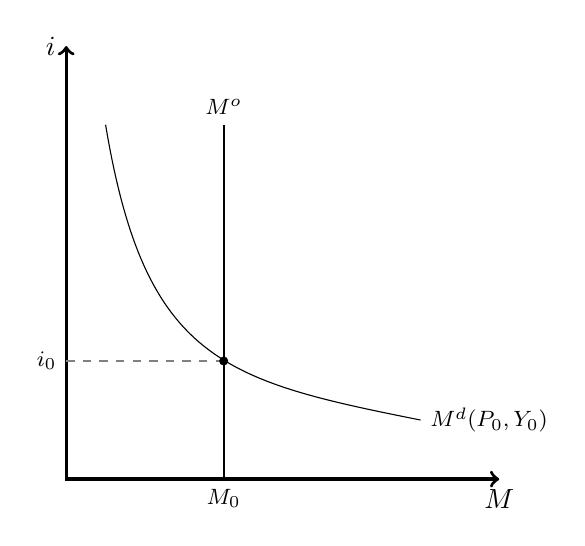
\begin{tikzpicture}[scale=0.5]
                    \draw[very thick,<->] (0,11) node[left]{$i$}--(0,0)--(11,0) node[below]{$M$};
                    \draw[thin] (1,9).. controls (2,3) and (4, 2.5) .. (9, 1.5) node [right]{\footnotesize $M^{d} (P_0,Y_0)$};
                    \draw[thick](4, 0)--(4, 9) node [above]{\footnotesize $M^{o}$};
                    \draw[thick,gray, dashed](0,3)--(4,3);
                    \node[left] at (0,3) {\footnotesize $i_0$};
                    \node[below] at (4,0) {\footnotesize $M_0$};
                    \draw[fill](4,3) circle [radius =0.1];
                \end{tikzpicture}
            \end{center}
        \end{figure}
    \end{center} 
\end{frame}

\begin{frame}{Movimientos de la demanda de dinero}

\begin{columns}
    \column{0.4\textwidth}
    Si aumenta el producto de $Y_0$ a $Y_1$, la demanda de dinero aumenta y presiona a la tasa de interés a la suba: \\ \vspace{2mm}
    \footnotesize
    \centering
    Hay exceso de demanda de dinero a la tasa $i_0$ \\  $\downarrow$ \\ la gente convierte depósitos en dinero \\ $\downarrow$ \\ cae la oferta de FP \\ $\downarrow$ \\ la tasa de interés sube para equilibrar el mercado de crédito.
    
    \column{0.6\textwidth}
    \begin{center}
        \begin{figure}[H]
        \begin{center}
        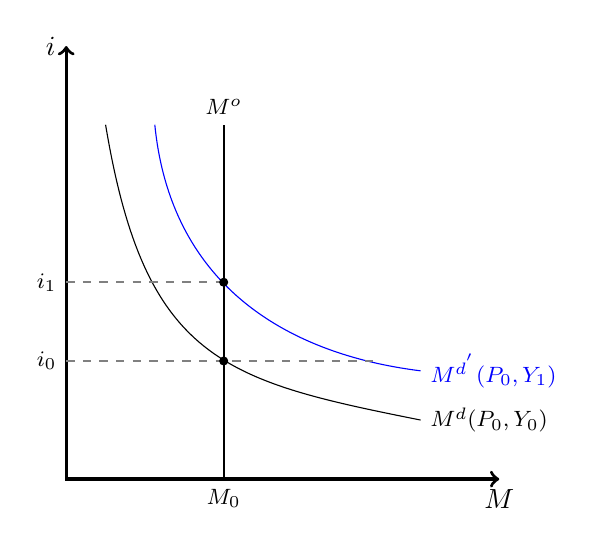
\begin{tikzpicture}[scale=0.5]
        \draw[very thick,<->] (0,11) node[left]{$i$}--(0,0)--(11,0) node[below]{$M$};
        \draw[thin] (1,9).. controls (2,3) and (4, 2.5) .. (9, 1.5) node [right]{\footnotesize $M^{d} (P_0, Y_0)$};
        \draw[thin, blue] (2.25,9).. controls (2.75,4) and (7, 3) .. (9, 2.75) node [right]{\footnotesize $M^{d^{'}} (P_0, Y_1)$};
        \draw[thick](4, 0)--(4, 9) node [above]{\footnotesize $M^{o}$};
        \draw[thick,gray, dashed](0,3)--(7.8,3);
        \node[left] at (0,3) {\footnotesize $i_0$};
        \draw[thick,gray, dashed](0,5)--(4,5);
        \node[left] at (0,5) {\footnotesize $i_1$};
        \node[below] at (4,0) {\footnotesize $M_0$};
        \draw[fill](4,3) circle [radius =0.1];
        \draw[fill](4,5) circle [radius =0.1];
        \end{tikzpicture}
        \end{center}
        \end{figure}
    \end{center} 

    \end{columns}
\end{frame}


\begin{frame}{Movimientos de la oferta de dinero}
    \begin{columns}
    \column{0.4\textwidth}
    Si el Banco Central emite dinero, la oferta de dinero se desplaza a la derecha y genera una baja de la tasa de interés: \\ \vspace{2mm}
    \footnotesize
    \centering
    Hay exceso de oferta de dinero a la tasa $i_0$ \\  $\downarrow$ \\ la gente lo deposita \\ $\downarrow$ \\ sube la oferta de FP \\ $\downarrow$ \\ la tasa de interés cae para equilibrar el mercado de crédito.

    \column{0.6\textwidth}
    \begin{center}
    \begin{figure}[h!]
    \begin{center}
        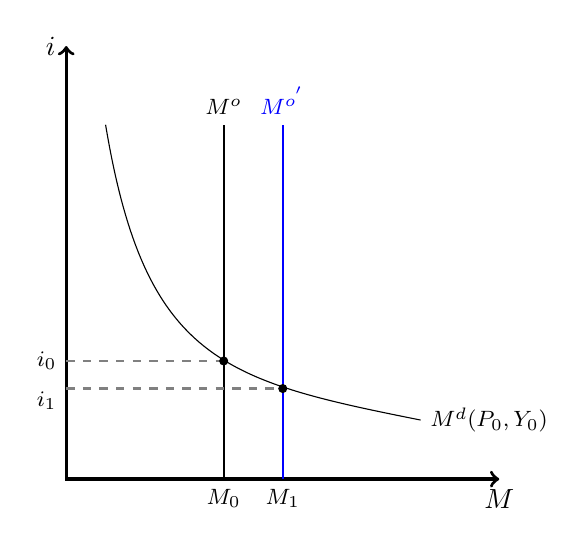
\begin{tikzpicture}[scale=0.5]
        \draw[very thick,<->] (0,11) node[left]{$i$}--(0,0)--(11,0) node[below]{$M$};
        \draw[thin] (1,9).. controls (2,3) and (4, 2.5) .. (9, 1.5) node [right]{\footnotesize $M^{d} (P_0, Y_0)$};
        \draw[thick](4, 0)--(4, 9) node [above]{\footnotesize $M^{o}$};
        \draw[thick, blue](5.5, 0)--(5.5, 9) node [above]{\footnotesize $M^{o^{'}}$};
        \draw[thick,gray, dashed](0,3)--(4,3);
        \node[left] at (0,3) {\footnotesize $i_0$};
        \draw[thick,gray, dashed](0,2.3)--(5.5,2.3);
        \node[left] at (0,2) {\footnotesize $i_1$};
        \node[below] at (4,0) {\footnotesize $M_0$};
        \node[below] at (5.5,0) {\footnotesize $M_1$};
        \draw[fill](4,3) circle [radius =0.1];
        \draw[fill](5.5,2.3) circle [radius =0.1];
        \end{tikzpicture}
    \end{center}
    \end{figure}
    \end{center} 
    \end{columns}
\end{frame}

\begin{frame}{Mercado de dinero}
    \begin{itemize}
        \item En el esquema clásico la cantidad de dinero determina la inflación.
        \item Acá estamos suponiendo que los precios estan fijos, por ende en este esquema keynesiano los movimientos en la cantidad de dinero determinan la tasa de interés.
        \item La mayoría de los bancos centrales fijan la tasa, pero es lo mismo.    
    \end{itemize}
\end{frame}


\begin{frame}{Funcionamiento del mercado monetario}
    \begin{center}
        \begin{figure}[H]
            \renewcommand{\figurename}{Figure}
            \begin{center}
                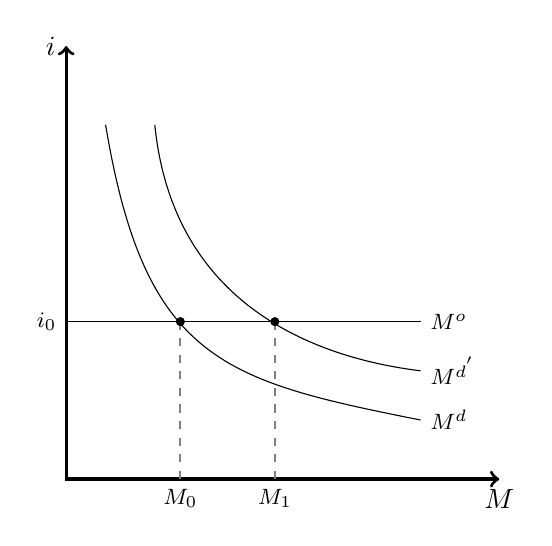
\begin{tikzpicture}[scale=0.5]
                    \draw[very thick,<->] (0,11) node[left]{$i$}--(0,0)--(11,0) node[below]{$M$};
                    \draw[thin] (0,4)--(9,4) node[right] {\footnotesize $M^{o}$};
                    \draw[thin] (1,9).. controls (2,3) and (4, 2.5) .. (9, 1.5) node [right]{\footnotesize $M^{d}$};
                    \draw[thin] (2.25,9).. controls (2.75,4) and (7, 3) .. (9, 2.75) node [right]{\footnotesize $M^{d^{'}}$};
                    \node[left] at (0,4) {\footnotesize $i_0$};
                    \draw[thick,gray, dashed](2.9,0)--(2.9,4);
                    \draw[thick,gray, dashed](5.3,0)--(5.3,4);
                    \node[below] at (2.9,0) {\footnotesize $M_0$};
                    \node[below] at (5.3,0) {\footnotesize $M_1$};
                    \draw[fill](2.9,4) circle [radius =0.1];
                    \draw[fill](5.3,4) circle [radius =0.1];
                \end{tikzpicture}
            \end{center}
        \end{figure}
    \end{center}
\end{frame}

\begin{frame}{Tasas de interés}
    
    \begin{itemize}
        \item Hasta el momento no explicitamos la distinción entre tasa de interés nominal y real.
        \item Tasa de interés nominal $i_t$
        \begin{itemize}
            \item ¿Cómo cambia, en términos de una moneda en particular, el valor de lo que presto o pido prestado? \\
            \item Un préstamo de \$V este año genera unos rendimientos de \$(1 + $i_t$)V el próximo año
        \end{itemize}
        \item Tasa de interés real $r_t$
        \begin{itemize}
            \item ¿Qué pasa si hay inflación?
            \item Tasas de interés expresadas en términos de una canasta de bienes (\textbf{corregida por inflación})
            \item Tasa que le importa a las personas sin ilusión monetaria
        \end{itemize}
    \end{itemize}
\end{frame}

\begin{frame}{Pensando en la relación}
\small
    \begin{itemize}
        \item Supongamos que invierto $\$100$ hoy ($t$) y la tasa de interés nominal  es $i=10\%$. ¿Cuánto obtengo mañana? 
        \[100 \times (1+i_t)= 100 \times (1+10\%)=110\]
        Este es el valor en pesos futuros. Pero eso no nos dice nada sobre qué podemos comprar con ese dinero si los precios también suben...
        \item ¿Cómo corregimos por inflación? Hagamos un paréntesis: si un producto cuesta $\$100$ y la inflación es 10\%, el año que viene cuesta:
        \[100 \times (1 + \pi) = 100 \times 1{,}10 = 110\]
        Es decir, los $\$110$ de mañana son $\$100$ a precios de hoy:
        \[100=\frac{110}{(1 + \pi)}\]
        Dividir por $1 + \pi$ es la forma de traer los pesos del futuro a precios actuales.
        \item Dado el ejemplo, los $\$100$ invertidos se convierten en $110$ (por $i=10\%$), pero si los precios también suben 10\% ($\pi=10\%$), entonces no ganamos poder adquisitivo $\rightarrow$ la tasa de interés real es 0\%. 
    \end{itemize}
\end{frame}


\begin{frame}
\frametitle{Intereses e inflación}
\begin{itemize}
    \item Por ende, la relación entre las tasas de interés y la inflación esperada es

        \[1+r_t=\frac{(1+i_t)}{(1+\pi_{t+1}^{e})}\]

    \item Suponiendo que el valor de las variables no es demasiado grande... $\frac{(1+x)}{(1+y)} \approx 1 + x - y $
    \item ... obtenemos la ecuación de Fisher: 

        \[r_t \approx i_t - \pi_{t+1}^{e}\]

        \[i_t \approx r_t + \pi_{t+1}^{e}\]

    \item Entender que ambas tasas estan relacionadas nos permite entender la relación entre el mercado monetario y el mercado de crédito.
    \end{itemize}
\end{frame}


\begin{frame}{Seba y Franco}
    \begin{itemize}
        \item Seba le pidió a Franco \$100 prometiendo pagar \$110, entonces la tasa nominal de interés es:
        \begin{center}
            $i_{HOY}=\frac{\$110 - \$100}{\$100} * 100 = 10\%$
        \end{center}
            \vspace{2mm}
        \item Si la tasa de inflación esperada para mañana es 5\%, entonces la tasa de interés real es: \\
        \begin{center}
            $r_{HOY} = i_{HOY}-\pi_{\text{MAÑANA}}^{e}$ \\
            \vspace{2mm}
            $r_{HOY} = 10\%-5\% $ \\
            \vspace{2mm}
            $r_{HOY} = 5\%$
        \end{center}
    \end{itemize}
\end{frame}

\begin{frame}{Antes de continuar}
    \begin{itemize}
        \item Vamos a ver la interrelación de los dos mercados suponiendo que los cambios en la cantidad de dinero \textbf{no son permanentes} (por ende no producen \textit{inflación esperada}).
        \item ¿Por qué podemos hacer esto?
        \begin{itemize}
            \item Para simplificar 
            \item Porque estamos pensando en el corto plazo y entendemos que hay ciertas rigideces que permiten que no se ajusten los precios.
            \item Porque para los clásicos aumentos en la cantidad de dinero no tienen efectos reales y por ende no van a ser utilizados como política económica.
        \end{itemize}
        \item De esa forma, la relación que establecimos previamente nos dice que podemos ver ambos mercados solo con la tasa de interés nominal.
    \end{itemize}
\end{frame}

\begin{frame}{Equilibrio: Mercado monetario y de crédito}
    \begin{center}
        \begin{figure}[H]
            \begin{center}
                \begin{minipage}[b]{0.45\textwidth}
                    \begin{center}
                        \begin{tikzpicture}[scale=0.4]
                            \draw[very thick,<->] (0,11) node[left]{$i$}--(0,0)--(11,0) node[below]{$FP$};
                            \node[] at(5,-1.5) {\underline{Mercado de Crédito}};
                            \node[left] at(0,6.2) {\scriptsize $i_0$};
                            \draw[thin](0.5,1.5)--(8.5,9) node [above] {\scriptsize $O_{FP}$};
                            \draw[thin](2.5,9)--(10.5,1.2) node [right] {\scriptsize $D_{FP}$};
                            \draw[fill] (5.4,6.15) circle [radius =0.11] node [below] {\scriptsize A};
                            \draw[thick,dashed,gray] (0,6.2)--(11,6.2);
                            \only<2->{
                                \node[left, blue] at(0,4.9) {\scriptsize $i_1$};
                                \draw[thin, blue](3,1.5)--(11,9) node [above] {\scriptsize $O_{FP}^{'}$};
                                \draw[fill, blue] (6.7,4.9) circle [radius =0.11] node [right] {\scriptsize B};
                                \draw[thick,dashed,gray] (0,4.9)--(6.7,4.9);
                            }
                            \only<3->{
                            \node[left, green!50!black] at(0,4.2) {\scriptsize $i_2$};
                            \draw[thin, green!50!black](4.5,1.5)--(11,7.5) node [above right] {\scriptsize $O_{FP}^{''}$};
                            \draw[fill, green!50!black] (7.6,4.2) circle [radius =0.11] node [below] {\scriptsize C};
                            \draw[thick,dashed,gray] (0,4.2)--(11,4.2);
                            }
                        \end{tikzpicture}
                    \end{center}
                \end{minipage}
                \begin{minipage}[b]{0.45\textwidth}
                    \begin{center}
                        \begin{tikzpicture}[scale=0.4]
                            \draw[very thick,<-] (0,11) node[left]{$i$}--(0,0);
                            \draw[very thick,->] (0,0)--(11,0) node[below]{$M$};
                            \node[] at(6,-1.5) {\underline{Mercado de Dinero}};
                            \draw[thin] (2.75, 9).. controls (3, 7) and (4,2.75) .. (9,2.25) node [right]{\footnotesize $M^{d} (P_0, Y_0)$};
                            \draw[thin](3.5,0)--(3.5,9) node [above]{\footnotesize $M^{o}$};
                            \draw[thin](7,0)--(7,9) node [above]{\footnotesize $M^{o^{'}}$};
                            \draw[fill] (3.5,6.25) circle [radius =0.11] node [below left] {\scriptsize A};
                            \node[below] at (3.5,0) {\footnotesize $M_0$};
                            \node[below] at (7,0) {\footnotesize $M_1$};
                            \draw [thin,gray,decorate,decoration={brace,amplitude=3pt},xshift=0pt,yshift=5pt](3.6,6.3) -- (7,6.3); 
                            \draw[thick,dashed,gray] (0,6.2)--(11,6.2);
                            \node[above] at(5.3,6.45) {\scriptsize Gap};
                            \only<2->{
                                \draw[thin, blue] (3.25, 9).. controls (4, 7) and (5,3) .. (9,3) node [right]{\footnotesize $M^{d^{'}} (P_0, Y_1)$};
                                \draw[fill, blue] (7,3.45) circle [radius =0.11] node[left] {\scriptsize B};
                            }
                            \only<3->{
                            \node [right, green!50!black] at (9,3.65) {\footnotesize $M^{d^{''}} (P_0, Y_2)$};
                            \draw[thin, green!50!black] (3.75, 9).. controls (4,7.75) and (5,4) .. (9,3.5);
                            \draw[fill, green!50!black] (6.9,4.2) circle [radius =0.11] node[above right] {\scriptsize C};
                            \draw[thick,dashed,gray] (0,4.2)--(11,4.2);
                            }
                        \end{tikzpicture}
                    \end{center}
                \end{minipage}
            \end{center}
        \end{figure}
    \end{center} 
    \begin{itemize}
        \footnotesize
        \item Partimos de un equilibrio A y aumenta la oferta de dinero. A la tasa $i_0$ hay exceso de oferta de dinero (Gap) \pause
        \item \textcolor{blue}{La gente deposita ese exceso y aumenta $O_{FP}$ $\rightarrow$ cae $i$ $\rightarrow$, $\uparrow C, \uparrow I$. Esto genera que $\uparrow Y$ y la demanda de dinero sea mayor. Pasamos a B} \pause
        \item \textcolor{green!50!black}{En tanto la tasa de interés del mercado de crédito se mantenga por encima de la del mercado de dinero, el proceso continua hasta llegar a C}
    \end{itemize} 
\end{frame}


\begin{frame}{Tres lecciones y un corolario}
    \begin{itemize}
        \item El proceso de ajuste no es lineal (por eso se las curvas se desplazan varias veces), por ende mientras el mercado de crédito tenga una tasa de interés distinta que la del mercado de dinero, el proceso de ajuste continua.
        \item El aumento en la cantidad de dinero disminuye la tasa de interés (podemos obviar el trasfondo del mercado de crédito)
        \item Si uno de los mercados está en equilibrio el otro también, por lo que nos alcanza con tener presente solo uno de los dos (Ley de Walras).
        \item De acá en más vamos a pensar en el mercado de dinero y en el mercado de bienes. Sabemos que ambos por detras tienen al mercado de crédito y al mercado de trabajo.
    \end{itemize}
\end{frame}




\end{document}



